\documentclass[14pt]{extbook}
\usepackage{multicol, enumerate, enumitem, hyperref, color, soul, setspace, parskip, fancyhdr} %General Packages
\usepackage{amssymb, amsthm, amsmath, latexsym, units, mathtools} %Math Packages
\everymath{\displaystyle} %All math in Display Style
% Packages with additional options
\usepackage[headsep=0.5cm,headheight=12pt, left=1 in,right= 1 in,top= 1 in,bottom= 1 in]{geometry}
\usepackage[usenames,dvipsnames]{xcolor}
\usepackage{dashrule}  % Package to use the command below to create lines between items
\newcommand{\litem}[1]{\item#1\hspace*{-1cm}\rule{\textwidth}{0.4pt}}
\pagestyle{fancy}
\lhead{Progress Quiz 9}
\chead{}
\rhead{Version A}
\lfoot{9541-5764}
\cfoot{}
\rfoot{Summer C 2021}
\begin{document}

\begin{enumerate}
\litem{
Construct the lowest-degree polynomial given the zeros below. Then, choose the intervals that contain the coefficients of the polynomial in the form $ax^3+bx^2+cx+d$.\[ \frac{-3}{4}, \frac{7}{4}, \text{ and } \frac{1}{5} \]\begin{enumerate}[label=\Alph*.]
\item \( a \in [71, 88], b \in [-99, -95], c \in [-89, -81], \text{ and } d \in [-25, -15] \)
\item \( a \in [71, 88], b \in [-222, -215], c \in [143, 147], \text{ and } d \in [-25, -15] \)
\item \( a \in [71, 88], b \in [-99, -95], c \in [-89, -81], \text{ and } d \in [16, 31] \)
\item \( a \in [71, 88], b \in [57, 67], c \in [-121, -119], \text{ and } d \in [16, 31] \)
\item \( a \in [71, 88], b \in [94, 102], c \in [-89, -81], \text{ and } d \in [-25, -15] \)

\end{enumerate} }
\litem{
Describe the end behavior of the polynomial below.\[ f(x) = 7(x - 7)^{4}(x + 7)^{7}(x - 3)^{2}(x + 3)^{2} \]\begin{enumerate}[label=\Alph*.]
\begin{multicols}{2}\item 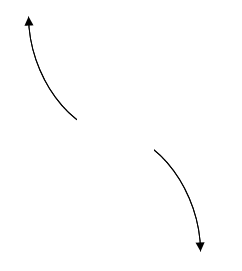
\includegraphics[width = 0.3\textwidth]{../Figures/polyEndBehaviorCopyAA.png}\item 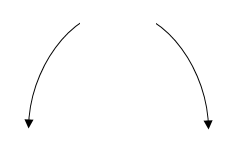
\includegraphics[width = 0.3\textwidth]{../Figures/polyEndBehaviorCopyBA.png}\item 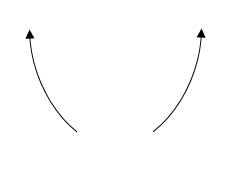
\includegraphics[width = 0.3\textwidth]{../Figures/polyEndBehaviorCopyCA.png}\item 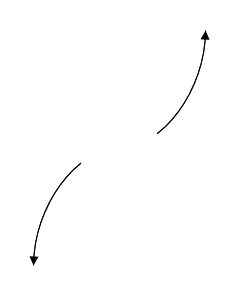
\includegraphics[width = 0.3\textwidth]{../Figures/polyEndBehaviorCopyDA.png}\end{multicols}\item None of the above.
\end{enumerate} }
\litem{
Construct the lowest-degree polynomial given the zeros below. Then, choose the intervals that contain the coefficients of the polynomial in the form $x^3+bx^2+cx+d$.\[ 5 - 4 i \text{ and } -4 \]\begin{enumerate}[label=\Alph*.]
\item \( b \in [3, 20], c \in [-0.68, 1.9], \text{ and } d \in [-168, -161] \)
\item \( b \in [-1, 4], c \in [5.04, 8.21], \text{ and } d \in [16, 23] \)
\item \( b \in [-6, -4], c \in [-0.68, 1.9], \text{ and } d \in [164, 166] \)
\item \( b \in [-1, 4], c \in [-1.45, 0.42], \text{ and } d \in [-20, -17] \)
\item \( \text{None of the above.} \)

\end{enumerate} }
\litem{
Which of the following equations \textit{could} be of the graph presented below?
\begin{center}
    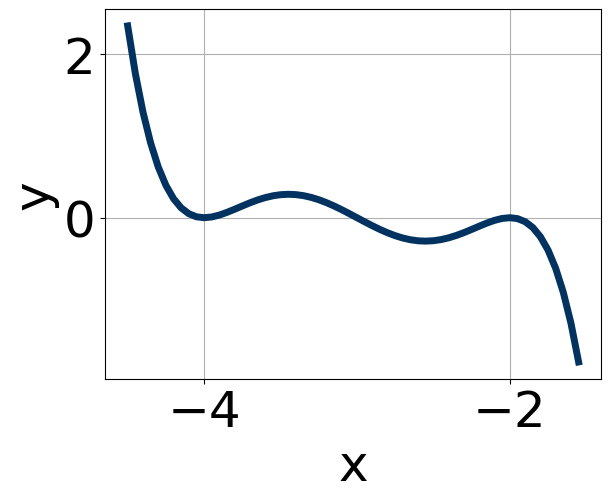
\includegraphics[width=0.5\textwidth]{../Figures/polyGraphToFunctionCopyA.png}
\end{center}
\begin{enumerate}[label=\Alph*.]
\item \( -13(x + 2)^{10} (x + 4)^{7} (x + 3)^{6} \)
\item \( 18(x + 2)^{10} (x + 4)^{6} (x + 3)^{10} \)
\item \( 16(x + 2)^{4} (x + 4)^{4} (x + 3)^{5} \)
\item \( -6(x + 2)^{10} (x + 4)^{6} (x + 3)^{5} \)
\item \( -15(x + 2)^{6} (x + 4)^{7} (x + 3)^{11} \)

\end{enumerate} }
\litem{
Describe the zero behavior of the zero $x = -8$ of the polynomial below.\[ f(x) = 6(x + 7)^{3}(x - 7)^{2}(x - 8)^{5}(x + 8)^{4} \]\begin{enumerate}[label=\Alph*.]
\begin{multicols}{2}\item 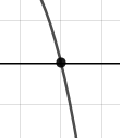
\includegraphics[width = 0.3\textwidth]{../Figures/polyZeroBehaviorCopyAA.png}\item 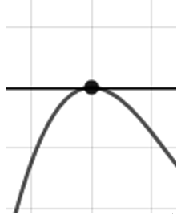
\includegraphics[width = 0.3\textwidth]{../Figures/polyZeroBehaviorCopyBA.png}\item 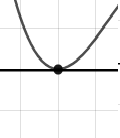
\includegraphics[width = 0.3\textwidth]{../Figures/polyZeroBehaviorCopyCA.png}\item 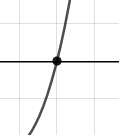
\includegraphics[width = 0.3\textwidth]{../Figures/polyZeroBehaviorCopyDA.png}\end{multicols}\item None of the above.
\end{enumerate} }
\litem{
Describe the zero behavior of the zero $x = -9$ of the polynomial below.\[ f(x) = -2(x + 9)^{6}(x - 9)^{9}(x - 8)^{2}(x + 8)^{5} \]\begin{enumerate}[label=\Alph*.]
\begin{multicols}{2}\item 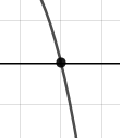
\includegraphics[width = 0.3\textwidth]{../Figures/polyZeroBehaviorAA.png}\item 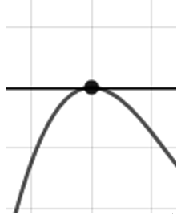
\includegraphics[width = 0.3\textwidth]{../Figures/polyZeroBehaviorBA.png}\item 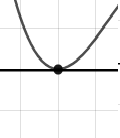
\includegraphics[width = 0.3\textwidth]{../Figures/polyZeroBehaviorCA.png}\item 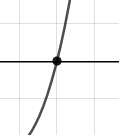
\includegraphics[width = 0.3\textwidth]{../Figures/polyZeroBehaviorDA.png}\end{multicols}\item None of the above.
\end{enumerate} }
\litem{
Describe the end behavior of the polynomial below.\[ f(x) = -4(x - 2)^{3}(x + 2)^{4}(x - 9)^{5}(x + 9)^{5} \]\begin{enumerate}[label=\Alph*.]
\begin{multicols}{2}\item 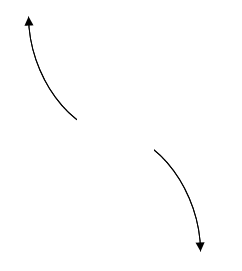
\includegraphics[width = 0.3\textwidth]{../Figures/polyEndBehaviorAA.png}\item 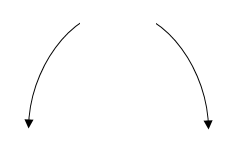
\includegraphics[width = 0.3\textwidth]{../Figures/polyEndBehaviorBA.png}\item 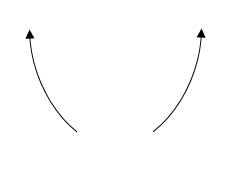
\includegraphics[width = 0.3\textwidth]{../Figures/polyEndBehaviorCA.png}\item 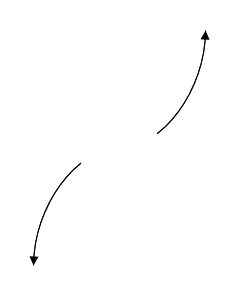
\includegraphics[width = 0.3\textwidth]{../Figures/polyEndBehaviorDA.png}\end{multicols}\item None of the above.
\end{enumerate} }
\litem{
Construct the lowest-degree polynomial given the zeros below. Then, choose the intervals that contain the coefficients of the polynomial in the form $x^3+bx^2+cx+d$.\[ -3 + 2 i \text{ and } 1 \]\begin{enumerate}[label=\Alph*.]
\item \( b \in [-6.2, -2.7], c \in [7, 14], \text{ and } d \in [10, 14] \)
\item \( b \in [1.3, 5.6], c \in [7, 14], \text{ and } d \in [-16, -7] \)
\item \( b \in [-0.3, 3.3], c \in [-2, 3], \text{ and } d \in [-5, 0] \)
\item \( b \in [-0.3, 3.3], c \in [-6, -1], \text{ and } d \in [0, 3] \)
\item \( \text{None of the above.} \)

\end{enumerate} }
\litem{
Construct the lowest-degree polynomial given the zeros below. Then, choose the intervals that contain the coefficients of the polynomial in the form $ax^3+bx^2+cx+d$.\[ \frac{-5}{4}, \frac{-3}{4}, \text{ and } 5 \]\begin{enumerate}[label=\Alph*.]
\item \( a \in [15, 19], b \in [42, 52], c \in [-151, -140], \text{ and } d \in [68, 80] \)
\item \( a \in [15, 19], b \in [-48, -41], c \in [-151, -140], \text{ and } d \in [68, 80] \)
\item \( a \in [15, 19], b \in [-48, -41], c \in [-151, -140], \text{ and } d \in [-76, -69] \)
\item \( a \in [15, 19], b \in [-94, -79], c \in [23, 34], \text{ and } d \in [68, 80] \)
\item \( a \in [15, 19], b \in [-119, -111], c \in [173, 179], \text{ and } d \in [-76, -69] \)

\end{enumerate} }
\litem{
Which of the following equations \textit{could} be of the graph presented below?
\begin{center}
    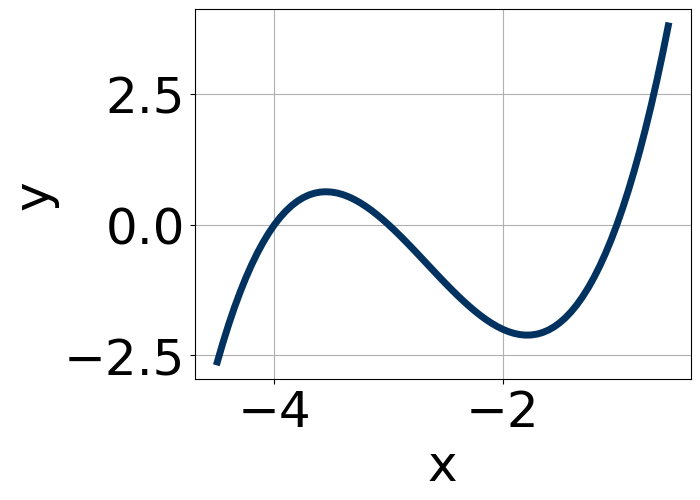
\includegraphics[width=0.5\textwidth]{../Figures/polyGraphToFunctionA.png}
\end{center}
\begin{enumerate}[label=\Alph*.]
\item \( 5(x + 1)^{8} (x + 3)^{4} (x + 4)^{5} \)
\item \( -17(x + 1)^{4} (x + 3)^{5} (x + 4)^{5} \)
\item \( 10(x + 1)^{11} (x + 3)^{7} (x + 4)^{11} \)
\item \( 5(x + 1)^{4} (x + 3)^{11} (x + 4)^{11} \)
\item \( -9(x + 1)^{7} (x + 3)^{11} (x + 4)^{9} \)

\end{enumerate} }
\end{enumerate}

\end{document}